\documentclass[a4paper, 12pt]{article}
\usepackage{template/sleek-settings}

% DEFAULT MARDKOWN SETUP

\RequirePackage[
    unicode=true,
    breaklinks=true,
    pdfusetitle,
    linktoc=page,
            colorlinks=true,
        linkcolor=black,
        citecolor=blue,
        urlcolor=blue,
    ]{hyperref}

\usepackage{color}
\usepackage{fancyvrb}
\newcommand{\VerbBar}{|}
\newcommand{\VERB}{\Verb[commandchars=\\\{\}]}
\DefineVerbatimEnvironment{Highlighting}{Verbatim}{commandchars=\\\{\}}
% Add ',fontsize=\small' for more characters per line
\usepackage{framed}
\definecolor{shadecolor}{RGB}{248,248,248}
\newenvironment{Shaded}{\begin{snugshade}}{\end{snugshade}}
\newcommand{\AlertTok}[1]{\textcolor[rgb]{0.94,0.16,0.16}{#1}}
\newcommand{\AnnotationTok}[1]{\textcolor[rgb]{0.56,0.35,0.01}{\textbf{\textit{#1}}}}
\newcommand{\AttributeTok}[1]{\textcolor[rgb]{0.77,0.63,0.00}{#1}}
\newcommand{\BaseNTok}[1]{\textcolor[rgb]{0.00,0.00,0.81}{#1}}
\newcommand{\BuiltInTok}[1]{#1}
\newcommand{\CharTok}[1]{\textcolor[rgb]{0.31,0.60,0.02}{#1}}
\newcommand{\CommentTok}[1]{\textcolor[rgb]{0.56,0.35,0.01}{\textit{#1}}}
\newcommand{\CommentVarTok}[1]{\textcolor[rgb]{0.56,0.35,0.01}{\textbf{\textit{#1}}}}
\newcommand{\ConstantTok}[1]{\textcolor[rgb]{0.00,0.00,0.00}{#1}}
\newcommand{\ControlFlowTok}[1]{\textcolor[rgb]{0.13,0.29,0.53}{\textbf{#1}}}
\newcommand{\DataTypeTok}[1]{\textcolor[rgb]{0.13,0.29,0.53}{#1}}
\newcommand{\DecValTok}[1]{\textcolor[rgb]{0.00,0.00,0.81}{#1}}
\newcommand{\DocumentationTok}[1]{\textcolor[rgb]{0.56,0.35,0.01}{\textbf{\textit{#1}}}}
\newcommand{\ErrorTok}[1]{\textcolor[rgb]{0.64,0.00,0.00}{\textbf{#1}}}
\newcommand{\ExtensionTok}[1]{#1}
\newcommand{\FloatTok}[1]{\textcolor[rgb]{0.00,0.00,0.81}{#1}}
\newcommand{\FunctionTok}[1]{\textcolor[rgb]{0.00,0.00,0.00}{#1}}
\newcommand{\ImportTok}[1]{#1}
\newcommand{\InformationTok}[1]{\textcolor[rgb]{0.56,0.35,0.01}{\textbf{\textit{#1}}}}
\newcommand{\KeywordTok}[1]{\textcolor[rgb]{0.13,0.29,0.53}{\textbf{#1}}}
\newcommand{\NormalTok}[1]{#1}
\newcommand{\OperatorTok}[1]{\textcolor[rgb]{0.81,0.36,0.00}{\textbf{#1}}}
\newcommand{\OtherTok}[1]{\textcolor[rgb]{0.56,0.35,0.01}{#1}}
\newcommand{\PreprocessorTok}[1]{\textcolor[rgb]{0.56,0.35,0.01}{\textit{#1}}}
\newcommand{\RegionMarkerTok}[1]{#1}
\newcommand{\SpecialCharTok}[1]{\textcolor[rgb]{0.00,0.00,0.00}{#1}}
\newcommand{\SpecialStringTok}[1]{\textcolor[rgb]{0.31,0.60,0.02}{#1}}
\newcommand{\StringTok}[1]{\textcolor[rgb]{0.31,0.60,0.02}{#1}}
\newcommand{\VariableTok}[1]{\textcolor[rgb]{0.00,0.00,0.00}{#1}}
\newcommand{\VerbatimStringTok}[1]{\textcolor[rgb]{0.31,0.60,0.02}{#1}}
\newcommand{\WarningTok}[1]{\textcolor[rgb]{0.56,0.35,0.01}{\textbf{\textit{#1}}}}




% Make links footnotes instead of hotlinks:
\renewcommand{\href}[2]{#2\footnote{\url{#1}}}


    \usepackage{blindtext}

\urlstyle{same}

% END OF DEFAULT MARKDOWN SETUP
% DYNAMIC VARIABLES

    \title{LSTAT2170 - Time series}

    \subtitle{Final Project}

    \author{\textsc{Lionel Lamy}   \\ Noma:  1294-1700  }

    \logo{resources/img/UCLouvain_Logo_Sciences.jpg}

    \institute{Université catholique de Louvain}

    \faculty{Louvain School of Statistics}



    \date{\today}

% END OF DYNAMIC VARIABLES

\begin{document}

    \maketitle
        {
     \setcounter{tocdepth}{3}
     \romantableofcontents
    }
        
    

    \hypertarget{introduction}{%
    \section{Introduction}\label{introduction}}
    
    In this project we will focus on the analysis of real data. These data
    are provided by the U.S. Natural Gas State Data and concern the
    aggregated monthly quantity of natural gas delivered to residential and
    commercial consumers (excluding vehicle fuel) in Florida. Aggregated on
    a monthly basis, the data are presented in millions of cubic feet
    (MMcf\footnote{\quad``Mcf'' means 1,000 cubic feet of natural gas;
      ``MMcf'' means 1,000 Mcf.}) and cover the period from January 1991 to
    August 1999.
    
    We will proceed to the beginning of this report with a first visual
    discovery of the dataset. Then, we will eventually apply a series of
    transformations to stabilize the variance, remove possible trends and
    seasonality. Next, we will analyze the autocorrelation and partial
    autocorrelation functions in order to have a first intuition on the type
    of model to fit. Following this, we will establish which model would be
    the most appropriate for our data and verify the insight of our choice
    by several methods such as a significance test of the coefficients, an
    analysis of the residuals (by a Portmanteau test) or the evaluation of
    the predictive capacity ``on sample''. The final objective is to be able
    to give a prediction interval for future values over roughly one year.
    
    \hypertarget{data-discovery}{%
    \section{Data discovery}\label{data-discovery}}
    
    \begin{center}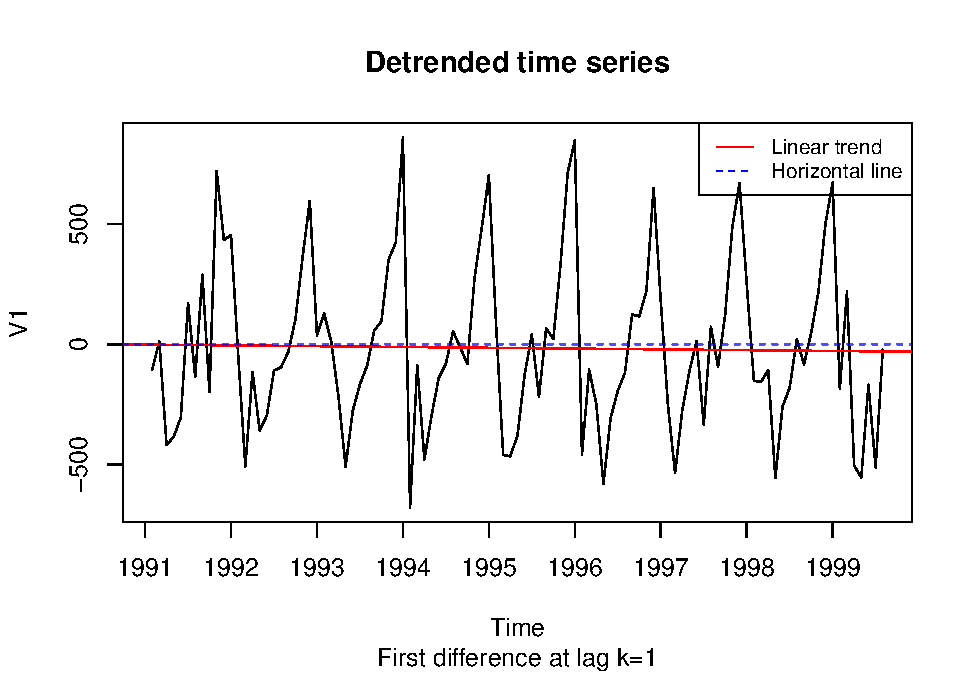
\includegraphics[width=0.8\linewidth]{resources/figs/unnamed-chunk-1-1} \end{center}
    
    In the graph above, we can observe an almost perfect seasonality with
    maximum values during the months of January and minimum from June to
    August. These results are hardly surprising given the nature of the
    data. Indeed, it seems normal that a greater quantity of gas is used in
    January (as it it the coldest month in Florida\footnote{\quad Source:
      \href{weather-us.com/en/florida-usa-climate}{weather-us.com}}) and
    that gas consumption decreases during summer.
    
    Looking at the trend line, we notice that from 1996 onwards the quantity
    delivered seems to decrease. We will try to keep this in mind when
    trying to predict future values.
    
    \begin{center}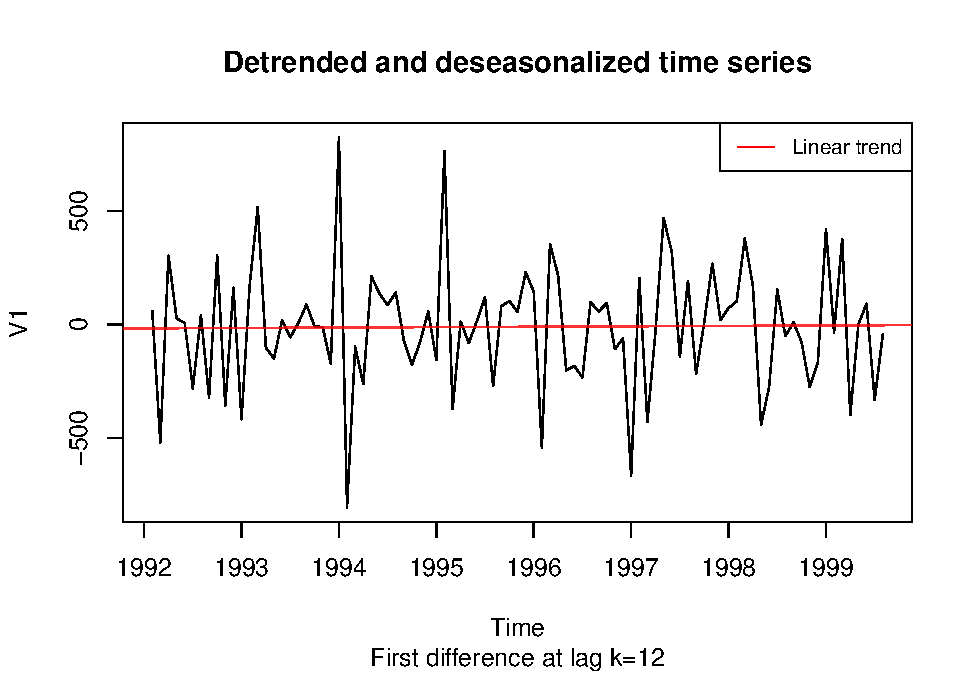
\includegraphics[width=0.8\linewidth]{resources/figs/unnamed-chunk-2-1} \end{center}
    
    \hypertarget{model-selection}{%
    \section{Model selection}\label{model-selection}}
    
    \hypertarget{section}{%
    \subsection{}\label{section}}
    
    \hypertarget{section-1}{%
    \subsection{}\label{section-1}}
    
    \hypertarget{conclusion}{%
    \section{Conclusion}\label{conclusion}}
    
    \newpage
    \appendix
    
    \hypertarget{appendix}{%
    \section{Appendix}\label{appendix}}
    
    \hypertarget{code}{%
    \subsection{Code}\label{code}}
    
    \bigskip
    \begin{mdframed}[style=thicc, frametitle=Note, frametitlebackgroundcolor=black!30]
      For reproducibility purposes, the complete R project containing the source code and the results is available on https://github.com/lamylio/LSTAT2170-Project.
    \end{mdframed}
    
    \begin{Shaded}
    \begin{Highlighting}[numbers=left,,]
    \CommentTok{# Import facility functions}
    \KeywordTok{source}\NormalTok{(}\StringTok{"./resources/scripts/fonctionsSeriesChrono.R"}\NormalTok{)}
    
    \KeywordTok{source}\NormalTok{(}\StringTok{"./resources/scripts/custom_plots.R"}\NormalTok{)}
    \KeywordTok{source}\NormalTok{(}\StringTok{"./resources/scripts/custom_timeseries.R"}\NormalTok{)}
    
    \CommentTok{# Import the gas dataset}
    \NormalTok{gas =}\StringTok{ }\KeywordTok{read.table}\NormalTok{(}\StringTok{"./resources/data/gasflorida.txt"}\NormalTok{, }\DataTypeTok{header =}\NormalTok{ F)}
    \NormalTok{gas =}\StringTok{ }\KeywordTok{ts}\NormalTok{(gas, }\DataTypeTok{start=}\DecValTok{1991}\NormalTok{, }\DataTypeTok{frequency =} \DecValTok{12}\NormalTok{)}
    
    \CommentTok{# Define some useful variables}
    \NormalTok{gas.attributes =}\StringTok{ }\KeywordTok{attributes}\NormalTok{(gas)}\OperatorTok{$}\NormalTok{tsp}
    \NormalTok{gas.start =}\StringTok{ }\NormalTok{gas.attributes[}\DecValTok{1}\NormalTok{]}
    \NormalTok{gas.end =}\StringTok{ }\NormalTok{gas.attributes[}\DecValTok{2}\NormalTok{]}
    \NormalTok{gas.freq =}\StringTok{ }\NormalTok{gas.attributes[}\DecValTok{3}\NormalTok{]}
    \end{Highlighting}
    \end{Shaded}


\end{document}
